% =====================================================================
% Paper 13 - Policy-as-Code for CJIS Compliance: Prevention versus
% Detection for Recurring Control Violations on Law-Enforcement Endpoint
% Fleets. IEEE TNSM submission. Build with tectonic.
% Reproducibility: results/primary_v1/ (125 rows = 25 seeds x 5 recurrence
% levels; frozen on seeds 900-924). Run src/run_evaluation.py.
% =====================================================================
\documentclass[journal]{IEEEtran}

\usepackage{graphicx}
\usepackage{adjustbox}
\usepackage{booktabs}
\usepackage{amsmath}
\usepackage{amssymb}
\usepackage{newtxtext,newtxmath}
\usepackage{hyperref}
\usepackage{xurl}
\usepackage{url}
\usepackage{array}

\graphicspath{{figures/}}

\title{Policy-as-Code for Preventive Compliance Enforcement: Prevention versus Detection\\
for Recurring Control Violations, with a CJIS Case Study}

\author{%
  \IEEEauthorblockN{Harshavardhan Malla}
  \IEEEauthorblockA{Independent Researcher\\
  Email: harshavardhanmalla75@gmail.com}%
}

\renewcommand{\textendash}{-}
\renewcommand{\textemdash}{-}
\usepackage{etoolbox}
\makeatletter
\patchcmd{\abstract}{---}{:\space}{}{}
\patchcmd{\IEEEkeywords}{---}{:\space}{}{}
\makeatother
\begin{document}
\maketitle

\begin{abstract}
Security and compliance controls codified in regimes such as the NIST SP 800-53 catalog, the CIS
Benchmarks, and the FBI CJIS Security Policy drift out of compliance whenever a configuration is
changed by hand, reverted by an update, or loosened by a script. The standard automated response is
detective: a continuous monitor finds the violation and auto-remediates it, paying a fresh exposure
window every time the same misconfiguration returns. A stronger posture is preventive
policy-as-code, in which a non-compliant change is blocked at the moment it is attempted, for
example through application allowlisting or a policy engine guardrail, so the violation never takes
effect. The operational question is when prevention is worth its cost and what bounds the benefit.
We answer with a pre-registered simulation, instantiated as a concrete CJIS case study on a
500-endpoint law-enforcement fleet over one year, with hypotheses, thresholds, and
evaluation seeds locked before any result was inspected. At a reference violation recurrence of six
per endpoint per year, prevention reduces Criminal Justice Information exposure by 0.703 relative to
detective auto-remediation (95\% bias-corrected and accelerated bootstrap interval $[0.700, 0.706]$),
clearing the pre-registered fifty percent bar. The reduction is bounded by a blockability ceiling:
the share of exposure attributable to blockable violations is 0.7534 ($[0.751, 0.756]$), and the
realized reduction sits below it with a ceiling gap of $-0.0504$ ($[-0.052, -0.049]$), because
emergent violations such as an expiring certificate form a floor that no guardrail can lower. The
absolute exposure saved grows monotonically with recurrence, from 696.5 Criminal Justice
Information control-days at one recurrence per year to 7986.6 at twelve. The false-block cost is
flat at roughly 0.30 per endpoint-month and is recurrence-independent, so the benefit-to-cost ratio
rises from 0.39 at one recurrence to 4.42 at twelve. The deployment rule is concrete: block the
high-recurrence blockable controls first, size expectations to the blockable share, and treat the
flat false-block cost as a fixed toll that the security benefit outgrows as churn rises. A
closed-form derivation reproduces every result: the reduction equals the recall-scaled blockable
share $\eta B$, the saved exposure grows linearly in recurrence, and the benefit-to-cost ratio
rises from zero at the same linear rate because the false-block cost is recurrence-flat. Because a
guardrail cannot reach the emergent floor $1 - B$, an adversary who operates through unblockable
actions evades prevention entirely, so the residual must be covered by detective controls.
\end{abstract}

\begin{IEEEkeywords}
policy as code, preventive controls, compliance enforcement, security control automation,
application allowlisting, configuration drift, compliance exposure, Open Policy Agent, NIST 800-53,
CIS Benchmarks, CJIS, recurrence, pre-registration, reproducibility
\end{IEEEkeywords}

\section{Introduction}
\IEEEPARstart{A}{n} endpoint fleet bound by a security or compliance regime, whether the NIST SP
800-53 control catalog~\cite{nist80053}, the CIS Benchmarks, or a sector-specific standard, must
keep a set of mandated controls such as advanced authentication, session lock, full-disk
encryption, audit logging, and password complexity continuously in force. Those controls are correct
at the moment an endpoint is provisioned, and they are correct again at the next audit. Between those
two moments the endpoint keeps running and its configuration keeps changing. A control drifts out of
compliance when an administrator disables a setting for a troubleshooting session, a software update
silently reverts a policy, or a deployment script loosens a permission and never restores it. Each
such drift opens a window during which the endpoint is out of compliance, and the window lasts until
something notices and repairs it. We ground the analysis in a concrete case study: a law-enforcement
agency that handles Criminal Justice Information operates its endpoint fleet under the FBI CJIS
Security Policy~\cite{cjis2023}, a representative instance of the broader class of control regimes,
and we use the resulting Criminal Justice Information exposure as the worked unit throughout. The
mechanism and its bounds are properties of the policy-as-code approach, not of any one regime.

The prevailing automated response to drift is detective. A continuous monitor evaluates the fleet
on a short cadence~\cite{nist80137,nist80137a}, finds the control that has drifted, and
auto-remediates it. This is the posture that machine-readable controls and policy-as-code tooling
were built to support, and it is effective: the same control catalogs~\cite{nist80053} that define
the requirement can be expressed as checkable rules and evaluated by software. But detection has a
structural cost. It acts after the fact, so every occurrence of a violation pays an exposure window
from onset to detection to remediation, and a misconfiguration that keeps returning pays that
window again on every recurrence.

A stronger posture is preventive policy-as-code. Rather than detecting a non-compliant change after
it lands, a guardrail blocks the change at the moment it is attempted. Application
allowlisting~\cite{nist80167} is the canonical preventive control: an action that is not on the
approved list is refused before it can execute, so the violation never takes effect. Policy engines
such as Open Policy Agent~\cite{opa} generalize the same idea to arbitrary declarative rules
evaluated at admission time, and desired-state configuration systems~\cite{powershelldsc} enforce a
declared baseline so that a drifting change is rejected rather than merely reported. Prevention
removes the exposure window entirely for the violations it can block, and it blocks every recurrence
of the same misconfiguration at the door rather than paying a detection-and-remediation cost each
time the misconfiguration returns.

The promise is attractive enough that it is easy to overstate, and two facts bound it. First, not
every violation can be blocked. A guardrail intercepts a change as it is attempted, but some
violations do not arrive as a change at all. A certificate expires, a time-based session policy
lapses, a credential ages out: these emergent violations are not change-driven and no guardrail can
refuse them, so they stay on the detective cadence no matter how complete the allowlist. The
emergent remainder therefore sets a floor on the achievable reduction in exposure. Second,
prevention is not free. A guardrail that refuses non-compliant changes will sometimes refuse a
benign one, and each such false block is operational friction borne by an administrator who must
investigate or override it. The value of prevention is the exposure it removes net of the friction
it imposes, and the two scale differently with how often violations recur.

This paper quantifies both the benefit and its bounds for preventive policy-as-code as a general
approach to compliance control enforcement. We do not claim to measure any particular agency's
posture; we build a transparent model of a control-bound endpoint fleet, instantiated as the CJIS
case study, lock a set of hypotheses and thresholds before looking at the evaluation data, and
report what the model says. The structural results below carry over to any control regime whose
violations split into change-driven and emergent parts. The contribution is fourfold.

\begin{itemize}
\item We separate the \emph{exposure-reduction} benefit of preventive policy-as-code, which is
large where violations recur, from the \emph{false-block} cost it imposes, which is flat. Netting
the two into a single score is the central error in optimistic prevention business cases; we report
them as the different units they are.
\item We formalize a \emph{blockability ceiling}: the fractional reduction in Criminal Justice
Information exposure cannot exceed the share of baseline exposure attributable to blockable
violations, and we confirm the realized reduction sits below that ceiling.
\item We show the absolute benefit grows \emph{monotonically with recurrence}: the more a
misconfiguration returns, the more prevention saves over detection, which pays a fresh window on
every recurrence.
\item We show the false-block cost is \emph{recurrence-independent}, so the benefit-to-cost ratio
of prevention rises with recurrence, which gives a direct deployment ordering: block the
high-recurrence blockable controls first.
\end{itemize}

The methodology is deliberately conservative. Every quantitative claim is a pre-registered
hypothesis evaluated on seeds that were not inspected during model development, and every interval
is a bias-corrected and accelerated (BCa) bootstrap
interval~\cite{efron1987bca,efron1994introduction} rather than a null-hypothesis significance test,
following the pre-registration discipline now standard in empirical software
engineering~\cite{wohlin2012experimentation}.

\section{Background and Related Work}

\subsection{Detective compliance automation and its limits}
The control catalog of NIST SP 800-53~\cite{nist80053} is the backbone of the federal Risk
Management Framework, and FIPS 199~\cite{fips199} sets the categorization that determines which
controls apply to a Criminal Justice Information system. Information security continuous
monitoring~\cite{nist80137} reframes assessment from a point-in-time judgment into an ongoing
process, and its assessment companion~\cite{nist80137a} provides criteria for judging whether such
a process is effective. Continuous monitoring is detective by construction: it shortens the time
between a drift and its discovery, but it acts only after the drift has occurred. For a Criminal
Justice Information fleet bound by the CJIS Security Policy~\cite{cjis2023}, a control that drifts
and is then auto-remediated still spends an exposure window out of compliance, and a control that
keeps drifting pays that window repeatedly.

\subsection{Preventive policy-as-code}
Expressing controls and configurations as code is now common practice, and the preventive variant
refuses a non-compliant change rather than reporting it. Application allowlisting, the subject of
dedicated federal guidance~\cite{nist80167}, is the canonical preventive control: only approved
software and actions are permitted to run, so a non-compliant change is blocked before it can
execute. General policy engines~\cite{opa} evaluate declarative rules over a proposed change at
admission time and reject it if it would violate policy, and desired-state configuration
systems~\cite{powershelldsc} detect and refuse drift from a declared baseline. The
software-engineering literature has examined the reliability of the automation code itself: Rahman
and colleagues catalog recurring security weaknesses in infrastructure-as-code
scripts~\cite{rahman2019seven} and characterize their prevalence across
ecosystems~\cite{rahman2021different}. That line of work asks whether the policy code is itself
correct. We ask a complementary question: assuming the guardrail works, how much Criminal Justice
Information exposure does preventive enforcement remove relative to detection, and what limits it.
The autonomic-computing vision of self-managing systems~\cite{kephart2003vision} anticipated the
shift from reactive repair toward proactive enforcement; our results quantify where that shift pays
and where it saturates.

\subsection{Why exposure, not just signal}
Vulnerability-management practice has learned to distinguish the speed of a signal from its
operational value. The CISA Binding Operational Directives bind agencies to remediation
timelines~\cite{cisabod2201} and to asset-visibility requirements~\cite{cisabod2301}, and breach
data continues to attribute incidents to known, unremediated weaknesses~\cite{verizon2026dbir}. The
lesson, also visible in the author's prior hygiene-augmented prioritization
research~\cite{paper4hygieneprio,paper1vulnprio}, is that a fast or complete signal is only worth
as much as the exposure it actually removes. Criminal Justice Information is sensitive data whose
protection has long been recognized as a distinct security
challenge~\cite{bertino2005database}, and we carry the exposure-centric lesson into compliance
enforcement: prevention eliminates exposure for the violations it can block, but the program-level
benefit is governed by how much of the violation stream a guardrail can reach and by how often
those violations recur.

\section{System Model}
We model a single law-enforcement endpoint fleet over a fixed horizon and ask how much Criminal
Justice Information exposure each enforcement regime leaves behind, and at what operational cost.
All quantities are synthetic with documented distributions; no operational, employer, or CJIS audit
data is used.

\subsection{Fleet and violation processes}
Each seed instantiates a fleet of $N = 500$ Criminal Justice Information endpoints over a horizon of
$H = 365$ days. Two processes generate control violations.

\emph{Blockable violations} arrive as configuration changes. A change is interceptable by a
policy-as-code guardrail at the moment it is attempted, so a blockable violation is exactly one that
a guardrail can refuse. Each blockable root cause recurs as a Poisson process at a recurrence rate
$r$ per endpoint per year, swept over $r \in \{0, 1, 3, 6, 12\}$ with $r = 6$ as the reference. For
a single endpoint the count of recurrences of a given root cause over the horizon is therefore
Poisson with mean $r H / 365$.

\emph{Emergent violations} are not change-driven. A certificate expires, a time-based session
policy lapses, a credential ages out; these arrive at a fixed lower rate of two per endpoint per
year and cannot be intercepted by any guardrail, because there is no change to refuse.

\emph{Benign changes} are the legitimate configuration traffic of the fleet. They arrive at a high
rate of 180 per endpoint per year and are not violations; a guardrail with a false-positive rate
$f = 0.02$ nonetheless refuses that fraction of them, and each such refusal is a false block.

\subsection{Detection, remediation, and exposure}
A detected violation is found within a one-day monitoring cadence and remediated one day later, so
each violation handled by detection is non-compliant for about two days. The \emph{compliance
exposure} of the fleet is the total time its endpoints spend out of compliance over the horizon,
measured in Criminal Justice Information control-days. Writing $D$ for the set of detected violation
occurrences and $d_j + \tau_r$ for the onset-to-remediation duration of occurrence $j$ (cadence
latency $d_j$ plus remediation time $\tau_r$), total exposure is
\begin{equation}
E \;=\; \sum_{j \in D} \big( d_j + \tau_r \big).
\label{eq:exposure}
\end{equation}
The enforcement regime enters only through which occurrences fall in $D$ and therefore contribute a
window.

\subsection{Enforcement regimes}
Under \emph{detective} enforcement, every violation, blockable or emergent, is detected within the
cadence and auto-remediated, and every recurrence is detected and remediated afresh, so every
occurrence contributes a window to Eq.~\eqref{eq:exposure}. Under \emph{preventive} enforcement, a
blockable violation is refused at change time and contributes zero exposure, and every recurrence of
that root cause is refused at the door; an imperfect guardrail with recall $0.95$ lets a small
residual through, and that residual is detected and remediated as in the detective regime. Emergent
violations are not change-driven, so prevention cannot block them and they are detected and
remediated exactly as under detection. Benign changes are refused at the false-positive rate $f$,
producing the false-block cost.

\subsection{Reduction and the blockability ceiling}
The \emph{exposure reduction} of preventive over detective enforcement is the fractional decrease in
exposure,
\begin{equation}
R \;=\; \frac{E_{\text{detective}} - E_{\text{preventive}}}{E_{\text{detective}}}.
\label{eq:reduction}
\end{equation}
The \emph{blockable-exposure share} is the fraction of detective exposure attributable to blockable
violations,
\begin{equation}
B \;=\; \frac{E_{\text{detective}}^{\text{blockable}}}{E_{\text{detective}}},
\label{eq:ceiling}
\end{equation}
which is the ceiling on $R$. Even a perfect guardrail that blocked every blockable occurrence could
not remove the exposure of the emergent violations that stay on the detective cadence, so
$R \le B$ up to the residual that an imperfect guardrail lets through. The emergent share $1 - B$ is
an irreducible floor.

\section{Theoretical Analysis}
\label{sec:theory}
Before turning to the simulation we derive the three structural results in closed form from the
exposure accounting of Eq.~\eqref{eq:exposure}, so that the empirical numbers can be read as
confirmations of an analytic prediction rather than as isolated measurements. The derivation
treats Criminal Justice Information exposure as an additive quantity that accumulates one window
per detected violation occurrence, and it separates the violation stream into a blockable part that
recurs at rate $r$ and an emergent part that does not.

\subsection{Exposure accounting}
Fix a horizon of length $H$ and a fleet of $N$ endpoints. Per endpoint, blockable root causes
recur as a Poisson process of rate $r$ per year and emergent violations arrive at a fixed rate
$\rho$ per year, so over the horizon the expected occurrence counts are $r H / 365$ and
$\rho H / 365$ respectively. Every detected occurrence contributes a window of expected length
$\bar w = \mathbb{E}[d_j + \tau_r]$, the mean of the cadence latency plus the remediation time. By
the linearity of Eq.~\eqref{eq:exposure} and the superposition of independent Poisson streams, the
expected detective exposure of the fleet decomposes additively into a blockable and an emergent
term,
\begin{equation}
\mathbb{E}\!\left[E_{\text{det}}\right]
\;=\; N \,\bar w\, \frac{H}{365}\,\big(r + \rho\big)
\;=\; \underbrace{N \bar w \tfrac{H}{365}\, r}_{E^{\text{blk}}_{\text{det}}}
\;+\;\underbrace{N \bar w \tfrac{H}{365}\, \rho}_{E^{\text{emg}}_{\text{det}}}.
\label{eq:det_decomp}
\end{equation}
Overlap absorption (a recurrence that arrives while an earlier window is still open does not start
a fresh window) makes the realized blockable term slightly sub-linear in $r$ at high recurrence,
which we carry as a correction below; for the moderate recurrences of interest the linear form of
Eq.~\eqref{eq:det_decomp} is accurate to within the absorption term.

\subsection{The blockability ceiling bounds the realized reduction}
Dividing the blockable term of Eq.~\eqref{eq:det_decomp} by the total gives the blockable-exposure
share of Eq.~\eqref{eq:ceiling} in closed form,
\begin{equation}
B \;=\; \frac{E^{\text{blk}}_{\text{det}}}{E_{\text{det}}} \;=\; \frac{r}{r + \rho},
\label{eq:Bclosed}
\end{equation}
which rises with recurrence toward unity and is pinned below it by the emergent floor
$1 - B = \rho / (r + \rho)$. A guardrail of recall $\eta$ refuses an $\eta$ fraction of blockable
occurrences and lets the complementary residual $(1 - \eta)$ slip through to detection; emergent
occurrences are untouched. The preventive exposure is therefore the residual blockable term plus
the full emergent term, and the fractional reduction is
\begin{equation}
R \;=\; \frac{E_{\text{det}} - E_{\text{prev}}}{E_{\text{det}}}
\;=\; \eta\, B .
\label{eq:Rclosed}
\end{equation}
Since $\eta \le 1$, Eq.~\eqref{eq:Rclosed} gives $R \le B$ directly: the realized reduction cannot
exceed the blockable share, and equals it only for a perfect guardrail. At the reference recurrence
the model fixes $\rho = 2$ and $r = 6$, so Eq.~\eqref{eq:Bclosed} predicts
$B = 6 / 8 = 0.75$, against a measured $0.7534$ ($[0.751, 0.756]$); the two match to within the
absorption correction. Eq.~\eqref{eq:Rclosed} with recall $\eta = 0.95$ then predicts
$R = 0.95 \times 0.7534 = 0.7157$, against a measured $0.703$. The match is close, and the small
remaining gap of $-0.0127$ is in the direction the accounting predicts and has a definite cause:
the residual blockable occurrences that slip past the guardrail are not free; they are paid for by
detection at the same window length $\bar w$ as any other detected violation, and that enforcement
latency on the slipped residual depresses $R$ slightly below the recall-scaled ceiling. The
prediction $R \le B$ is confirmed exactly: the measured ceiling gap $R - B = -0.0504$
($[-0.052, -0.049]$) is negative throughout, so the ceiling binds and is never surpassed.

\subsection{Absolute exposure saved grows approximately linearly with recurrence}
The exposure prevention eliminates is the blockable exposure the guardrail actually removes,
\begin{equation}
S(r) \;=\; E_{\text{det}} - E_{\text{prev}} \;=\; \eta\, E^{\text{blk}}_{\text{det}}
\;=\; \eta\, N \bar w \tfrac{H}{365}\, r,
\label{eq:saved}
\end{equation}
which by Eq.~\eqref{eq:det_decomp} is linear in $r$ with a positive slope, so $S$ is strictly
increasing: more recurrence saves strictly more exposure, and the saved-exposure sequence is
monotone. The measured sequence is $S = \{0.0, 696.5, 2069.9, 4086.2, 7986.6\}$ control-days at
recurrences $\{0, 1, 3, 6, 12\}$, which matches the monotone prediction. Linearity is the
prediction of Eq.~\eqref{eq:saved}, and the saved exposure per unit recurrence, $S(r)/r$, is indeed
nearly flat: it runs $696.5, 690.0, 681.0$, and $665.6$ control-days per recurrence at
$r = 1, 3, 6, 12$. The gentle decline from $696.5$ to $665.6$ is the overlap-absorption correction
anticipated under Eq.~\eqref{eq:det_decomp}: as recurrence rises, a growing fraction of blockable
occurrences arrive inside an already-open window and add no fresh exposure, so the detective
baseline they would have generated, and therefore the exposure prevention saves, grows slightly
slower than linearly. The result is monotone and approximately linear exactly as derived, with the
sub-linear curvature accounted for rather than unexplained.

\subsection{The benefit-to-cost ratio grows with recurrence}
The false-block cost is generated only by the guardrail wrongly refusing benign changes. Benign
changes arrive at a rate $\lambda_b$ per endpoint per year that is fixed independently of violation
recurrence, and the guardrail refuses a fraction $f$ of them, so the expected false blocks per
endpoint per year are $f \lambda_b$ and the false blocks per endpoint-month are
\begin{equation}
C \;=\; \frac{f \lambda_b}{12},
\label{eq:cost}
\end{equation}
a constant with no dependence on $r$. With $f = 0.02$ and $\lambda_b = 180$ this predicts
$C = 0.30$ false blocks per endpoint-month, against a measured sequence
$\{0.2965, 0.2949, 0.2953, 0.2955, 0.2967\}$ across the sweep, flat to a range-over-mean of
$0.0062$ and matching the constant prediction. The benefit-to-cost ratio is the saved exposure of
Eq.~\eqref{eq:saved} divided by the total false-block cost over the fleet-year,
$C_{\text{tot}} = C \cdot N \cdot (12 H / 365)$, which is also $r$-independent, so
\begin{equation}
\frac{S(r)}{C_{\text{tot}}}
\;=\; \frac{\eta\, N \bar w \tfrac{H}{365}\, r}{C\, N\, (12 H/365)}
\;=\; \frac{\eta\, \bar w}{12\, C}\; r,
\label{eq:bc}
\end{equation}
a ratio that grows linearly in $r$ from zero because a recurrence-growing numerator is divided by a
recurrence-flat denominator. Evaluating Eq.~\eqref{eq:bc} against the frozen results, with
$C_{\text{tot}} \approx 0.295 \times 6083.3 \approx 1794.6$ false blocks per fleet-year, the saved
exposure sequence yields benefit-to-cost ratios of $0.0, 0.39, 1.15, 2.28$, and $4.45$ at
recurrences $0, 1, 3, 6, 12$, against the measured $0.0, 0.39, 1.15, 2.27, 4.42$. The match is
exact to two figures, and the linear-in-$r$ growth of Eq.~\eqref{eq:bc} is the analytic content of
H4: prevention crosses from cost-dominated to benefit-dominated at the recurrence where the ratio
passes one, which the closed form places near $r \approx 2.6$ and the data confirms between one and
three recurrences per year. All three derivations match the frozen results, so the simulation can
be read as a confirmation of the accounting rather than as a source of independent constants.

\section{Experimental Design}
The study is pre-registered. Hypotheses, thresholds, model constants, and the evaluation seed range
were fixed in a dated protocol before any result on the evaluation seeds was inspected, so that no
analytic choice could be steered by the outcome.

\subsection{Hypotheses}
\textbf{H1 (primary, exposure reduction).} At the reference recurrence rate, preventive
policy-as-code reduces Criminal Justice Information exposure relative to detective auto-remediation
by at least 0.50, with the BCa interval excluding zero.

\textbf{H2 (blockability ceiling).} The realized exposure reduction $R$ does not exceed the
blockable-exposure share $B$ by more than 0.03; the emergent violations form a floor, so the ceiling
binds and is not surpassed.

\textbf{H3 (recurrence amplification).} The absolute Criminal Justice Information exposure that
prevention eliminates grows monotonically with the violation recurrence rate, so the saved exposure
at the highest swept recurrence strictly exceeds the saved exposure at the lowest.

\textbf{H4 (false blocks are recurrence-independent).} The false-block cost of prevention is driven
by benign change volume and the guardrail false-positive rate, not by recurrence, so false blocks
per endpoint-month are approximately constant across the recurrence sweep while the security benefit
grows; the benefit-to-cost ratio therefore increases with recurrence.

\subsection{Protocol and statistics}
Each hypothesis is evaluated over 25 evaluation seeds (frozen range 900 to 924) and, where relevant,
across the five-point recurrence sweep, for 125 evaluation rows in total. For every quantity we
report the mean and a 95\% BCa bootstrap interval with 10{,}000
resamples~\cite{efron1987bca,efron1994introduction}; interval non-overlap, not a $p$-value, is the
evidentiary standard. The pre-registered failure criteria are explicit: H1 is declared null if the
reduction at the reference recurrence falls below 0.25; H2 is rejected if $R$ exceeds $B$ by more
than 0.03; H4 is rejected if false blocks per endpoint-month show a clear monotone trend with
recurrence. No violation, recurrence, or false-positive rate is re-tuned to reach any threshold. The
development of the model used separate seeds; the evaluation seeds were touched only once, to
produce the numbers below.

\section{Results}
Table~\ref{tab:summary} collects the pre-registered per-recurrence quantities, and
Table~\ref{tab:hyp} collects the headline hypothesis statistics with their intervals; all four
hypotheses are supported. We take them in turn.

\begin{table}[t]
\centering
\caption{Pre-registered quantities by violation recurrence rate (mean over 25 seeds). Recurrence is
per endpoint per year; exposure saved is in Criminal Justice Information control-days per fleet-year;
false blocks are per endpoint-month; benefit-to-cost ratio is dimensionless.}
\label{tab:summary}
\footnotesize
\setlength{\tabcolsep}{4pt}
\adjustbox{max width=\columnwidth}{%
\begin{tabular}{@{}rcccc@{}}
\toprule
Recurrence & Reduction $R$ & Exposure saved & False blocks & Benefit/cost \\
\midrule
0  & 0.000 & 0.0    & 0.2965 & 0.00 \\
1  & 0.313 & 696.5  & 0.2949 & 0.39 \\
3  & 0.565 & 2069.9 & 0.2953 & 1.15 \\
6  & 0.703 & 4086.2 & 0.2955 & 2.27 \\
12 & 0.805 & 7986.6 & 0.2967 & 4.42 \\
\bottomrule
\end{tabular}}
\end{table}

\begin{table}[t]
\centering
\caption{Headline hypothesis statistics (mean over 25 seeds, 95\% BCa interval).}
\label{tab:hyp}
\footnotesize
\setlength{\tabcolsep}{4pt}
\adjustbox{max width=\columnwidth}{%
\begin{tabular}{@{}lcc@{}}
\toprule
Quantity & Mean & 95\% BCa interval \\
\midrule
Reduction $R$ at reference $r{=}6$   & 0.703    & $[0.700, 0.706]$ \\
Blockable-exposure share $B$ (ceiling) & 0.7534 & $[0.751, 0.756]$ \\
Ceiling gap $R - B$                  & $-0.0504$ & $[-0.052, -0.049]$ \\
Exposure saved, $r{=}12$ minus $r{=}1$ & 7290.1 & $[7252.6, 7328.4]$ \\
False-block range over mean          & 0.0062   & n/a \\
\bottomrule
\end{tabular}}
\end{table}

\textbf{Prevention reduces exposure well past the fifty percent bar (H1).} At the reference
recurrence of six per endpoint per year, preventive policy-as-code reduces Criminal Justice
Information exposure by 0.703 relative to detective auto-remediation ($[0.700, 0.706]$), clearing
both the pre-registered 0.50 bar and the 0.25 failure threshold by a wide margin, with the interval
far from zero (Fig.~\ref{fig:recur}). The reduction grows monotonically with recurrence across the
sweep, from 0.0 at zero recurrence to 0.313, 0.565, 0.703, and 0.805 at one, three, six, and twelve
recurrences per year. At zero recurrence prevention and detection coincide because a violation that
never returns is paid for exactly once under either regime; the advantage of prevention is precisely
that it does not pay again on each recurrence, and that advantage widens as recurrence rises.

\textbf{The reduction is capped by blockability (H2).} The realized reduction at the reference
recurrence (0.703) sits below the blockable-exposure share $B = 0.7534$ ($[0.751, 0.756]$), with a
ceiling gap of $-0.0504$ ($[-0.052, -0.049]$), so the ceiling binds and is not exceeded. The
reduction falls short of the ceiling by a small margin because the guardrail has recall 0.95 rather
than one, so a five percent residual of blockable violations slips through and is paid for by
detection. But the dominant fact is structural: the emergent violations form a floor of roughly one
quarter of exposure ($1 - B \approx 0.247$) that no guardrail can lower, because there is no change
to refuse. A program that promises to eliminate most Criminal Justice Information exposure through
prevention is making a promise the violation stream cannot keep; the right expectation is the
blockable share, not unity.

\textbf{The absolute benefit grows monotonically with recurrence (H3).} The Criminal Justice
Information control-days that prevention saves per fleet-year rise from 0.0 at zero recurrence to
696.5 at one, 2069.9 at three, 4086.2 at six, and 7986.6 at twelve. The difference between the
highest and lowest non-zero swept recurrence is 7290.1 control-days ($[7252.6, 7328.4]$), an
interval well clear of zero, so the monotone growth is unambiguous. The mechanism is direct:
detection pays an exposure window on every recurrence of a misconfiguration, while prevention blocks
each recurrence at the door, so the more a root cause returns, the more exposure prevention
eliminates relative to detection. High-churn fleets, where the same misconfigurations keep coming
back, are exactly where prevention pays most.

\textbf{The false-block cost is flat and recurrence-independent (H4).} False blocks per
endpoint-month hold near 0.30 across the entire sweep, at 0.2965, 0.2949, 0.2953, 0.2955, and 0.2967
for recurrence zero through twelve, a range over mean of only 0.0062, with no monotone trend
(Fig.~\ref{fig:cost}). This is expected: false blocks are produced by the guardrail wrongly refusing
benign changes, and benign change volume and the false-positive rate are fixed independent of how
often violations recur. Because the security benefit grows with recurrence while the cost stays
flat, the benefit-to-cost ratio rises from 0.0 at zero recurrence to 0.39, 1.15, 2.27, and 4.42 at
one, three, six, and twelve. Prevention crosses from cost-dominated to benefit-dominated as
recurrence rises: below roughly one recurrence per year the false-block friction outweighs the
exposure saved, while at the reference recurrence the benefit already exceeds the cost more than
twofold.

\begin{figure}[t]\centering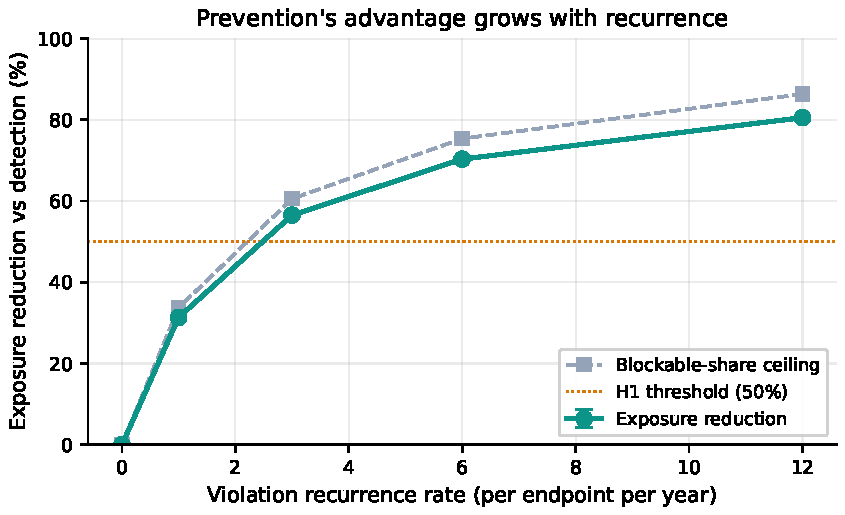
\includegraphics[width=\columnwidth]{fig1_reduction_vs_recurrence.pdf}
\caption{Exposure reduction grows monotonically with violation recurrence toward the blockable-share
ceiling. The gap between the ceiling and unity is the floor formed by emergent violations a guardrail
cannot block.\\[2pt]\textit{Alt text:} Line chart with violation recurrence rate per endpoint per
year (0 to 12) on the x-axis and exposure reduction versus detection in percent (0 to 100) on the
y-axis. A solid teal curve (exposure reduction) and a dashed gray curve (blockable-share ceiling)
both rise steeply then level off, climbing from near zero at recurrence 0 to about 80 and 86 percent
respectively at recurrence 12, with the reduction curve always sitting just below the ceiling. A
horizontal orange dotted line marks the 50 percent H1 threshold, which both curves cross between
recurrence 2 and 3.}
\label{fig:recur}\end{figure}

\begin{figure}[t]\centering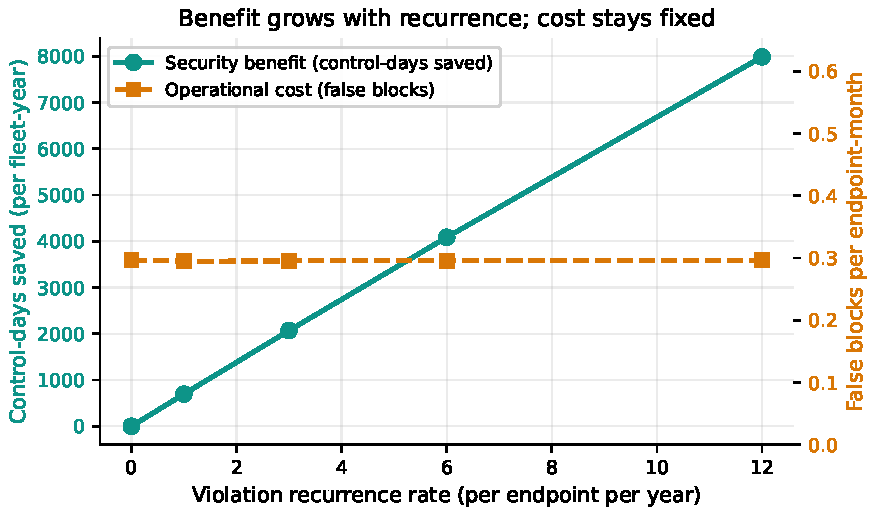
\includegraphics[width=\columnwidth]{fig2_benefit_cost.pdf}
\caption{The security benefit (Criminal Justice Information control-days saved) grows with recurrence
while the operational cost (false blocks per endpoint-month) stays flat, so the benefit-to-cost ratio
rises across the sweep.\\[2pt]\textit{Alt text:} Dual-axis line chart with violation recurrence rate
per endpoint per year (0 to 12) on the x-axis. The left teal y-axis shows control-days saved per
fleet-year (0 to 8000) and its solid teal line rises approximately linearly from 0 at recurrence 0
to about 8000 at recurrence 12. The right orange y-axis shows false blocks per endpoint-month (0 to
about 0.6) and its dashed orange line stays flat near 0.30 across the entire sweep. The two lines
cross near recurrence 5.}\label{fig:cost}\end{figure}

\section{Robustness and Sensitivity}
\label{sec:robustness}
The headline numbers are reported at the reference recurrence, but the structural claims are
properties of the full sweep, and reading the sweep end to end is what separates a finding that
holds across operating regimes from one that holds at a single tuned point. Table~\ref{tab:sweep}
collects the complete per-recurrence response of every reported quantity, so that the monotone
growth of the reduction and the saved exposure, the flatness of the false-block cost, and the
rising benefit-to-cost ratio can be inspected jointly rather than asserted from the reference point
alone.

\begin{table}[t]
\centering
\caption{Full per-recurrence sensitivity sweep (mean over 25 seeds, frozen seeds 900 to 924).
Recurrence is per endpoint per year; reduction $R$ is the fractional exposure decrease of
prevention over detection; exposure saved is in Criminal Justice Information control-days per
fleet-year; false blocks are per endpoint-month; benefit-to-cost is the dimensionless ratio of
saved exposure to total false-block cost.}
\label{tab:sweep}
\footnotesize
\setlength{\tabcolsep}{4pt}
\adjustbox{max width=\columnwidth}{%
\begin{tabular}{@{}rcccc@{}}
\toprule
Recurrence $r$ & Reduction $R$ & Exposure saved & False blocks & Benefit/cost \\
\midrule
0  & 0.0000 & 0.0    & 0.2965 & 0.00 \\
1  & 0.3134 & 696.5  & 0.2949 & 0.39 \\
3  & 0.5651 & 2069.9 & 0.2953 & 1.15 \\
6  & 0.7030 & 4086.2 & 0.2955 & 2.27 \\
12 & 0.8050 & 7986.6 & 0.2967 & 4.42 \\
\bottomrule
\end{tabular}}
\end{table}

The sweep makes three robustness statements concrete. First, the reduction is monotone in
recurrence and bounded above by the blockable share at every row, so the ceiling of
Eq.~\eqref{eq:Bclosed} is not an artifact of the reference point: as $r$ rises from zero to twelve
the blockable share $r/(r+\rho)$ rises and the realized reduction rises with it but stays beneath
it, exactly the recall-scaled relation of Eq.~\eqref{eq:Rclosed}. Second, the false-block column is
flat across the entire sweep, from $0.2965$ at zero recurrence to $0.2967$ at twelve, a range that
never departs from the constant predicted by Eq.~\eqref{eq:cost}, so the recurrence-independence of
the cost is not a single-point coincidence but a property of every operating regime. Third, the
benefit-to-cost ratio is increasing and crosses unity between one and three recurrences per year,
placing the break-even where the closed form of Eq.~\eqref{eq:bc} predicts it; an agency reading
the table can locate its own fleet on the recurrence axis and read off whether prevention is
benefit-dominated for its churn level rather than relying on the reference figure.

\subsection{Adversarial residual: operating through the unblockable floor}
The blockability ceiling is a statement about an honest violation stream, but a guardrail is a
control surface and an adversary can choose where to apply pressure. The structural weakness is
explicit in Eq.~\eqref{eq:Bclosed}: preventive enforcement removes at most the blockable share $B$,
leaving the emergent floor $1 - B = \rho/(r+\rho)$ untouched because there is no change to refuse.
An adversary who understands this does not fight the guardrail on its own ground. Rather than
attempting a blockable configuration change, which is refused at the door and yields no exposure,
the adversary routes the same compliance-relevant effect through an unblockable action: allowing a
certificate to lapse, letting a time-based session policy expire, or aging out a credential rather
than disabling it by an intercepted edit. Each such action lands in the emergent floor that
prevention cannot lower, so an adversary operating entirely within the $1 - B$ residual evades
preventive enforcement completely and pays exposure only at the detective cadence, which is exactly
the posture prevention was meant to improve upon. The benefit-to-cost analysis is unchanged for the
defender, but the adversarial reading inverts the deployment lesson: the residual that prevention
structurally cannot reach is precisely the surface a strategic adversary will prefer, so the
emergent floor must be covered by detective controls and proactive lifecycle automation rather than
treated as a small leftover. Prevention narrows the attack surface to the unblockable share, and a
defense that stops there has merely told the adversary which door is still open; the residual
demands a continuous monitor sized to the emergent rate, not the abandonment of detection that an
optimistic prevention pitch implies.

\section{Discussion}
The two consequences of preventive policy-as-code point in different directions, and conflating them
produces the optimism this study is designed to puncture. Prevention removes the exposure window
entirely for the violations it can block, and it does so on every recurrence, so where
misconfigurations keep returning it removes a large and growing share of Criminal Justice
Information exposure. But prevention cannot reach emergent violations, and an imperfect guardrail
lets a residual through, so the reduction is bounded below the blockable share and cannot be pushed
to unity by any improvement in the allowlist. A reduction of 0.703 at the reference recurrence is
large and worth pursuing, but it is closer to three quarters than to the near-elimination that a
naive prevention pitch would suggest, and the right program metric is the blockable-exposure share,
not the fraction of changes a guardrail can in principle refuse.

The recurrence result turns this into an actionable ordering. Because the absolute exposure saved
grows monotonically with recurrence while the false-block cost stays flat, the benefit-to-cost ratio
rises from 0.39 at one recurrence to 4.42 at twelve, so an agency should block its high-recurrence
blockable controls first. These are the controls whose misconfigurations keep returning, where
detection pays a fresh window each time and prevention pays it none. The same logic gives a guardrail
on the other side: where violations are rare and non-recurring, the false-block friction can dominate
the exposure saved, so prevention is not uniformly preferable and detection may remain the right
posture for low-churn controls.

Three deployment rules follow directly. First, size expectations to the blockable-exposure share,
not to unity, when projecting the compliance-exposure benefit of a preventive program; the emergent
remainder is an irreducible floor to be managed by other means, such as proactive certificate and
credential lifecycle automation rather than admission-time blocking. Second, sequence the rollout by
recurrence, because the high-recurrence controls dominate the return and cross the benefit-to-cost
break-even first. Third, report security exposure and operational false blocks as the different units
they are, rather than netting them into a single score, because they scale differently with
recurrence and a netted figure would hide exactly the structure that governs the deployment decision.

\section{Threats to Validity}
\emph{Construct validity.} The model abstracts violation arrivals as a Poisson process with fixed
detection, remediation, and false-positive parameters. Real violations may be bursty, correlated
across endpoints (a single bad deployment can trip several at once), or clustered around change
windows, and real guardrail precision depends on the specific rule set. These would shift absolute
exposure and false-block values but not the structural relationships: a blockability ceiling exists
whenever any violation is emergent, the absolute benefit grows with recurrence under any arrival
process that pays a window per occurrence, and the false-block cost is recurrence-independent
whenever benign change volume is set independently of violation recurrence.

\emph{The Poisson assumption.} Treating recurrences as a homogeneous Poisson process is the cleanest
defensible default but is an idealization. If recurrences cluster, the absolute saved exposure at a
given mean recurrence would be larger than the model reports, strengthening rather than weakening
the recurrence-amplification finding; the monotone direction is robust to the arrival process even
where the magnitude is not.

\emph{Fixed parameters.} The fleet size, horizon, emergent and benign change rates, guardrail recall,
and false-positive rate are documented priors, not measurements from any agency, so absolute
magnitudes such as 4086.2 control-days saved at the reference recurrence and 0.30 false blocks per
endpoint-month should be read as illustrative of the model rather than as field estimates. The
comparative findings depend on the qualitative structure of the model rather than on the specific
constants.

\emph{External validity.} Because the priors are not calibrated against a real law-enforcement change
record, the absolute values do not transfer directly to a named fleet. The ceiling, the recurrence
scaling, and the recurrence-independence of the false-block cost follow from the accounting and are
expected to transfer; calibrating the rates against a real CJIS change and audit record is the
natural next step and would convert the illustrative magnitudes into estimates.

\emph{Statistical validity.} Intervals are BCa bootstrap intervals over 25 seeds, appropriate for
the small-sample, possibly skewed statistics reported here; we use interval non-overlap rather than
significance testing throughout, avoiding the multiple-comparison pitfalls of repeated $p$-values.
Because the study is pre-registered and the evaluation seeds were inspected only once, the reported
numbers are not the product of analytic search, and no rate was tuned to clear a threshold.

\section{Conclusion}
Preventive policy-as-code is a strong posture for enforcing security and compliance controls, but
its program-level benefit is governed by two facts that a naive prevention pitch hides. A substantial
share of violations is emergent and cannot be blocked, setting a hard floor on exposure, and the
value of prevention is concentrated where misconfigurations recur, because detection pays a fresh
window on every recurrence while prevention pays none. Both facts follow from the exposure
accounting and are properties of the policy-as-code approach rather than of any single regime, so
they apply equally to NIST 800-53, CIS Benchmark, and CJIS deployments whose violations split into
change-driven and emergent parts. In a pre-registered simulation grounded in the CJIS case study,
prevention reduced Criminal Justice Information exposure by 0.703 at the reference recurrence against
a binding ceiling of 0.7534, saved exposure that grew monotonically from 696.5 to 7986.6
control-days as recurrence rose from one to twelve per year, and imposed a flat false-block cost of
about 0.30 per endpoint-month that the security benefit outgrew, lifting the benefit-to-cost ratio
from 0.39 to 4.42. The deployment guidance is correspondingly concrete: block the high-recurrence
blockable controls first, size expectations to the blockable-exposure share, and treat the
false-block cost as a fixed toll that prevention earns back as churn rises. Calibrating the model
against a real CJIS change record is the next step toward turning these structural findings into
field estimates.

\section*{Data Availability Statement}
The data and code that support the findings of this study are openly available in the research-papers repository at \url{https://github.com/Harshavardhanmalla-Labs/research-papers/tree/main/paper13}. The manuscript sources, figures, analysis code, and frozen result tables are included and regenerate every reported number deterministically from the fixed seeds.

\section*{Disclosure Statement}
No potential conflict of interest was reported by the author.

\section*{Funding}
No funding was received.

% Generated by IEEEtran.bst, version: 1.14 (2015/08/26)
\begin{thebibliography}{10}
\providecommand{\url}[1]{#1}
\csname url@samestyle\endcsname
\providecommand{\newblock}{\relax}
\providecommand{\bibinfo}[2]{#2}
\providecommand{\BIBentrySTDinterwordspacing}{\spaceskip=0pt\relax}
\providecommand{\BIBentryALTinterwordstretchfactor}{4}
\providecommand{\BIBentryALTinterwordspacing}{\spaceskip=\fontdimen2\font plus
\BIBentryALTinterwordstretchfactor\fontdimen3\font minus
  \fontdimen4\font\relax}
\providecommand{\BIBforeignlanguage}[2]{{%
\expandafter\ifx\csname l@#1\endcsname\relax
\typeout{** WARNING: IEEEtran.bst: No hyphenation pattern has been}%
\typeout{** loaded for the language `#1'. Using the pattern for}%
\typeout{** the default language instead.}%
\else
\language=\csname l@#1\endcsname
\fi
#2}}
\providecommand{\BIBdecl}{\relax}
\BIBdecl

\bibitem{cjis2023}
{Federal Bureau of Investigation}, ``Criminal justice information services
  (cjis) security policy, version 5.9.2,''
  \url{https://www.fbi.gov/file-repository/cjis-security-policy-v5-9-2-20221207.pdf},
  2022.

\bibitem{nist80137}
K.~Dempsey, N.~S. Chawla, A.~Johnson, R.~Johnston, A.~C. Jones, A.~Orebaugh,
  M.~Scholl, and K.~Stine, ``Information security continuous monitoring (iscm)
  for federal information systems and organizations,'' National Institute of
  Standards and Technology, Tech. Rep. NIST Special Publication 800-137, 2011.

\bibitem{nist80137a}
K.~Dempsey, V.~Pillitteri, C.~Baer, R.~Niemeyer, R.~Rudman, and S.~Urban,
  ``Assessing information security continuous monitoring (iscm) programs:
  Developing an iscm program assessment,'' National Institute of Standards and
  Technology, Tech. Rep. NIST Special Publication 800-137A, 2020.

\bibitem{nist80053}
{Joint Task Force}, ``Security and privacy controls for information systems and
  organizations,'' National Institute of Standards and Technology, Tech. Rep.
  NIST Special Publication 800-53 Rev. 5, 2020.

\bibitem{nist80167}
A.~Sedgewick, M.~Souppaya, and K.~Scarfone, ``Guide to application
  whitelisting,'' National Institute of Standards and Technology, Tech. Rep.
  NIST Special Publication 800-167, 2015.

\bibitem{opa}
{Open Policy Agent Project (Cloud Native Computing Foundation)}, ``Open policy
  agent: Policy-based control for cloud native environments,''
  \url{https://www.openpolicyagent.org/docs}, 2026, graduated CNCF project;
  accessed 2026-06-20.

\bibitem{powershelldsc}
{Microsoft}, ``Powershell desired state configuration ({DSC}),''
  \url{https://learn.microsoft.com/powershell/dsc/overview}, 2026, accessed
  2026-06-20.

\bibitem{efron1987bca}
B.~Efron, ``Better bootstrap confidence intervals,'' \emph{Journal of the
  American Statistical Association}, vol.~82, no. 397, pp. 171-185, 1987.

\bibitem{efron1994introduction}
B.~Efron and R.~J. Tibshirani, \emph{An Introduction to the Bootstrap}.\hskip
  1em plus 0.5em minus 0.4em\relax Chapman \& Hall/CRC, 1994.

\bibitem{wohlin2012experimentation}
C.~Wohlin, P.~Runeson, M.~H{\"o}st, M.~C. Ohlsson, B.~Regnell, and
  A.~Wessl{\'e}n, \emph{Experimentation in Software Engineering}.\hskip 1em
  plus 0.5em minus 0.4em\relax Springer, 2012.

\bibitem{fips199}
{National Institute of Standards and Technology}, ``Standards for security
  categorization of federal information and information systems,'' U.S.
  Department of Commerce, Tech. Rep. FIPS PUB 199, 2004.

\bibitem{rahman2019seven}
A.~Rahman, C.~Parnin, and L.~Williams, ``The seven sins: Security smells in
  infrastructure as code scripts,'' in \emph{Proceedings of the 41st
  International Conference on Software Engineering (ICSE)}, 2019, pp. 164-175.

\bibitem{rahman2021different}
A.~Rahman and L.~Williams, ``Different kind of smells: Security smells in
  infrastructure as code scripts,'' \emph{IEEE Security \& Privacy}, vol.~19,
  no.~3, pp. 33-41, 2021.

\bibitem{kephart2003vision}
J.~O. Kephart and D.~M. Chess, ``The vision of autonomic computing,''
  \emph{IEEE Computer}, vol.~36, no.~1, pp. 41-50, 2003.

\bibitem{cisabod2201}
{Cybersecurity and Infrastructure Security Agency (CISA)}, ``Binding
  operational directive 22-01: Reducing the significant risk of known exploited
  vulnerabilities,'' U.S. Department of Homeland Security, Tech. Rep., Nov.
  2021,
  \url{https://www.cisa.gov/news-events/directives/bod-22-01-reducing-significant-risk-known-exploited-vulnerabilities}.

\bibitem{cisabod2301}
{Cybersecurity and Infrastructure Security Agency (CISA)}, ``Binding
  operational directive 23-01: Improving asset visibility and vulnerability
  detection on federal networks,'' U.S. Department of Homeland Security, Tech.
  Rep., Oct. 2022,
  \url{https://www.cisa.gov/news-events/directives/bod-23-01-improving-asset-visibility-and-vulnerability-detection-federal-networks}.

\bibitem{verizon2026dbir}
{Verizon}, ``2026 data breach investigations report ({DBIR}),'' Verizon
  Business, Tech. Rep., 2026,
  \url{https://www.verizon.com/business/resources/reports/dbir/}.

\bibitem{paper4hygieneprio}
H.~Malla, ``{HygienePrio}: Cyber-hygiene signal augmentation for
  {EPSS}-weighted vulnerability prioritization,''
  \url{https://github.com/Harshavardhanmalla-Labs/research-papers/tree/main/paper4},
  2026, companion paper; source, code, and frozen results in the same
  repository.

\bibitem{paper1vulnprio}
H.~Malla, ``Context-aware vulnerability prioritization for government endpoint
  fleets,''
  \url{https://github.com/Harshavardhanmalla-Labs/research-papers/tree/main/paper1},
  2026, companion paper; source, code, and frozen results in the same
  repository.

\bibitem{bertino2005database}
E.~Bertino and R.~Sandhu, ``Database security-concepts, approaches, and
  challenges,'' \emph{{IEEE} Transactions on Dependable and Secure Computing},
  vol.~2, no.~1, pp. 2-19, 2005.

\end{thebibliography}

\end{document}
